\documentclass[12pt,a4paper]{article}

\usepackage[left=20mm, right=20mm, top=20mm]{geometry} % to set up page formatting
\usepackage[skip=10pt]{parskip} % spacing in between paragraphs
\usepackage{graphicx} % Required for inserting images
\usepackage{amsmath} % Required for flexibility in mathematical equations
\usepackage{amssymb} % Required for certain math symbols e.g. E[.]
\usepackage{natbib} % Required for bibliography and citations
\usepackage{enumitem} % Required to remove gap between items in list
\usepackage{tikz} % Required to build tikz diagrams
\usepackage{xcolor} % to access colors in tikz diags
\usepackage{hyperref} % for web links

\title{Modelling and optimising the housing of homeless populations: ten month PhD review}
\author{Graham Burgess}
\date{October 2024}

\begin{document}

\maketitle

\begin{abstract}
Modelling and optimisation are popular tools for supporting resourcing and capacity decisions in healthcare and homeless settings. We show how deterministic optimisation with a fluid flow model can support long-term capacity planning for a homeless care setting in the San Francisco Bay Area, California. Models of multi fidelity, including stochastic simulation, are available in this setting, and the solution space is integer-ordered. We therefore explore both multi fidelity and integer-ordered simulation optimisation methods and discuss potential research contributions at the intersection of these active fields of research.
\end{abstract}

\section{Introduction}

Homelessness is a growing problem faced by communities worldwide. An example is Alameda County in the San Francisco Bay area, California, where approximately $8000$ people experienced homelessness in $2021$ alone. Decision makers within these communities typically have some leverage over how relevant resources are allocated to help alleviate homelessness. In Alameda County, the local government must split their resources between emergency shelter and permanent social housing. Shelter is relatively cheap and quick to set up. It provides a safer alternative to street homelessness but does not provide a stable long-term living situation for its residents. Permanent social housing is more expensive than shelter and can take longer to set up, but it does offer the stable long-term living situationd that homelessness people need to improve their quality of life. Building capacity to alleviate homelessness takes time, especially since funds are typically available in varying amounts from year to year. Decision makers in communities like Alameda County must therefore make good time-varying capacity planning decisions to reduce homelessness now and in the future.

Operational research (OR) methods offer helpful tools to support such public sector decision-making. Optimisation helps decision-making by looking for a feasible solution which performs best across a (potentially infinite) set of alternative feasible solutions. To do this, a model of the performance of a solution is needed, and the quality of the model affects the quality of the subsequent optimisation results. We can model the homelessness care system as a queue. Individual clients arrive and if there is no space in shelter, they wait in an unsheltered queue. Once they are finished in shelter, they can only leave when housing becomes available. Once in housing they stay for some time before leaving for good or rejoining the queue for shelter. 

The most accurate model of this queueing system is a high-fidelity stochastic simulation model. In this case, one can only estimate the performance of a solution and the subsequent optimisation falls in the realm of simulation optimisation (SO). There are different SO methods for different types of problem (which we later discuss) but the issue of limited computational resources pervades all SO methods. This issue stems from from the fact that a stochastic simulation is typically computationally expensive to run, and many simulation replications are required to be confident of a solution's performance, given the associated uncertainty.

As is common in queueing systems, lower fidelity models such as analytical queueing models offer a computationally cheaper alternative to stochastic simulation. They also offer helpful alternative perspectives on the dynamics of a queueing system. The drawback is that these models are typically less accurate, given the necessary assumptions which must be made. If one only uses a low-fidelity deterministic model to evaluate the performance of a solution, optimisation falls in the realm of deterministic optimisation. Performing this deterministic optimisation can be a helpful first step in the decision-making process. However, there is more we can do with our low fidelity models. Multi-fidelity simulation optimisation (MFSO) enables low-fidelity models to be used alongside high fideltiy stocahstic simulation in a SO algorithm which reduces the computational burden and therefore enables an optimal solution to be found more efficiently. Novel MFSO methods will be the main topic of this PhD research.

This document is organised as follows: in Section \ref{lit-rev} we briefly review relevant literature on modelling and optimisation in homeless care settings and healthcare settings. There are many similarities between these two areas but the latter is more widely studied in the literature. We also review relevant SO methods including MFSO. In Sections \ref{models} and \ref{do} we discuss the main content of the PhD research to date. Section \ref{models} introduces three models of multi-fidelity for homeless care systems. Section \ref{do} introduces an optimisation formualation which addresses the time-varying capacity planning problem and we solve this problem in a determinsitc setting. In Section \ref{uncert} we discuss how different types of uncertainty affect our decision-making process, and this discussion motivates the need for simulation optimisation. In Section \ref{mfso} we discuss relevant interesting gaps in the current MFSO literature which the remainder of this PhD research seeks to address.

\newpage

\section{Literature Review} \label{lit-rev}

\subsection{Modelling and optimisation in healthcare settings}

Modelling hospital waiting lists using stochastic simulation e.g. \cite{wood2022supporting} and using stocks and flows e.g. \cite{worthington1991hospital}. Optimisation such as \cite{argyris2022fair} who balance efficiency and fairness in healthcare provision. 

\subsection{Modelling and optimisation in homeless care settings}

Simulation modelling of homeless care system in Alameda County \citep{singham2023discrete} and of shelters for runaway homeless youths (RHYs) \citep{kaya2022discrete}. Optimisation such as \cite{kaya2022improving} who minimise the cost of matching demand with supply for RHYs who require beds and support services.

\subsection{Simulation optimisation (SO)}

\subsubsection{Overview of SO methods}

\begin{itemize}[noitemsep]
\item Discrete SO: ranking \& selection, adaptive random search, integer-ordered.
\item Continuous SO: sample average approx, stochastic approx, meta models.
\end{itemize}

\subsubsection{Integer-ordered SO methods}
\begin{itemize} [noitemsep]
    \item Retrospective search with piecewise-linear interpolation and neighborhood enumeration (R-SPLINE) \citep{wang2013integer}.
    \item Discrete Stochastic Approximation \citep{lim2012stochastic}
    \item Gaussian Markov Random Fields \citep{l2019gaussian}
\end{itemize}

\subsubsection{Multi fidelity SO methods}

\begin{itemize}[noitemsep]
\item Using deterministic optimisation results to begin simulation optimisation e.g. \cite{jian2015introduction}.
\item Ordinal transformation with optimal sampling \citep{xu2016mo2tos}.
\item Modelling the error of a low-fidelity model
\begin{itemize}[noitemsep]
\item Polynomial error terms e.g. \cite{chong2018simulation}.
\item Gaussian Process error terms e.g. \cite{huang2006sequential}.
\end{itemize}
\item Multi-fidelity Expensive Black Box (Mf-EBB) Optimisation
\end{itemize}

\newpage

\section{Models of multi-fidelity} \label{models}

Here we introduce three models which we have developed for homeless care systems from low- to high-fidelity. Our low-fidelity model is a fluid flow model, which assumes housing servers are always busy and treats flow in and out of the system like a liquid with a continuous-valued volume. Our medium-fidelity model is an $M_t/M/h_t$ queueing model which relaxes the server-always-busy assumption. We incorporate stochasticity and using a Markov chain analysis we can compute the expected number of people housed, sheltered and unsheltered at some point in time, given initial conditions. Our high-fidelity model is a discrete-event simulation model. Here, as well as caputuring stochasticity we are able to model additional real-world processes such as a tandem queueing system with shelter and housing servers, partial re-entry to the system and non-Markovian service time distributions. We now discuss each model in turn.

\subsection{Fluid flow model} \label{fluid-model}
%
We start by making some assumptions to allow a simple model to be appropriate. Given that the main purpose of shelter is to accommodate people waiting for housing, rather than to offer a particular service which is needed to proceed, it is reasonable to treat shelter as part of the queue for housing, with houses being the sole set of servers in the queueing system. We therefore would like to model the system illustrated in Figure \ref{fig:simple-q}. In an overloaded queueing system such as the homeless care system in Alameda County, it is reasonable to assume that housing servers are always busy. With this assumption, the service process becomes independent of the arrival process and it is then straightforward to separately compute the number of arrivals and service completions in some time period, given arrival and service rates, which may be non-stationary.
%
\tikzstyle{server} = [rectangle, rounded corners, minimum width=0cm, minimum height=1cm,text centered, draw=black, fill=teal!30]
\tikzstyle{empty} = [rectangle, draw=none, fill=none]
\tikzstyle{arrow} = [thick,->,>=stealth]
%
\begin{figure} 
  \begin{center}
    \begin{tikzpicture}
      \node (start) [empty] {};
      \node (shelter) [empty, right of=start, xshift=2cm] {};
      \node (housing) [server, right of=shelter, xshift=2.2cm] {Housing};
      \node (end) [empty, right of=housing, xshift=2.1cm] {};
      \draw [arrow] (start) -- node [above] {Unsheltered \hspace{0.5cm} Sheltered} (housing);
      \draw [arrow] (housing) -- node [above] {}(end);  
      \draw[dashed] (3.0,-1) -- (3.0,1);
    \end{tikzpicture}
    \caption{Simple queueing system} \label{fig:simple-q}
  \end{center}
\end{figure}

We would like to track the number of housed, sheltered, and unsheltered people over time. The two main inputs to the model are a changing arrival rate over time, and a housing service rate which changes as housing is built.  Additionally, the amount of shelter space available to support the queue for housing may change over time. We ignore the randomness in the arrival process and the service process for homeless people entering and leaving the homeless care system. Instead we assume that ``fluid" flows into the system continuously at a rate $\lambda(t)$ and flows out at  rate $\mu(t) = \mu_{0}h(t)$ where $\mu_{0}$ is the service rate of a single housing server and $h(t)$ is the continuous-valued number of houses at time $t$. Given the initial number of people in the system $n_0$, at time $t$ we can calculate the subsequent number of people in the system, $n(t)$, as
%
\begin{equation*} \label{x_t}
n(t) = n_0 + \int_{0}^{t} \lambda(t) dt - \int_{0}^{t} \mu_0 h(t) dt.
\end{equation*}
%
We split the queue for housing into an unsheltered and a sheltered part. We denote by $s(t)$ the continuous-valued number of shelters at time $t$. The size of the unsheltered queue $u(t)$ is then 
%
\begin{align} 
u(t) & = n(t) - h(t) - s(t) \\
& = n_0 + \int_{0}^{t} \lambda(t) dt - \int_{0}^{t} \mu_0 h(t) dt - h(t) - s(t),
\label{u_t}
\end{align}
%
where we assume that capacities $h(t)$ and $s(t)$ are sufficiently small compared to the given arrival rate $\lambda(t)$ so that these resources are always full, and the use of a fluid flow model remains appropriate. In other words, the number of people housed and the number in shelter are the same as the housing and shelter capacities $h(t)$ and $s(t)$, respectively. In reality, there may be some friction in the system in that housing may be idle while units are experiencing turnover and the next person in the queue is being located, but this time can be incorporated into the service time distribution.

When analyzing the dynamics of the fluid flow model over a modeling horizon, we discretize time into days. We now let $\lambda_d, h^D_d, s^D_d$ and $u_d$ for all $d \in \{1,...,D\}$ be the discretized equivalents of $\lambda(t), h(t), s(t)$ and $u(t)$, respectively, where $D$ is the modeling horizon in days and is used as a superscript where we must later distinguish between daily and annual capacities. In order to evaluate an objective functions (which we describe in Section \ref{do}) we approximate (\ref{u_t}) with the sum 
%
\begin{align} \label{u_t_discrete}
u_d & = n_0 + \sum_{d'=1}^{d} \lambda_{d'} \delta t - \sum_{d'=1}^{d} \mu_0 h^D_{d'} \delta t - h^D_d - s^D_d, 
\end{align}
%
where $\mu_0$ is the daily service rate of a single housing unit and the stepsize $\delta t = 1 \text{ day}$. In Figure \ref{fig:ut-illustrative} we give an illustrative example of the dynamics of $u_d$ given by our fluid flow model, calibrated using realistic inputs for $n_0, \mu_0$ and $\lambda_d, h^D_d, s^D_d$ for all $d \in \{1,...,D\}$ which we take directly from \cite{singham2023discrete}. 
%
\begin{figure}[h!]%[ut-illustrative]
    \centering
    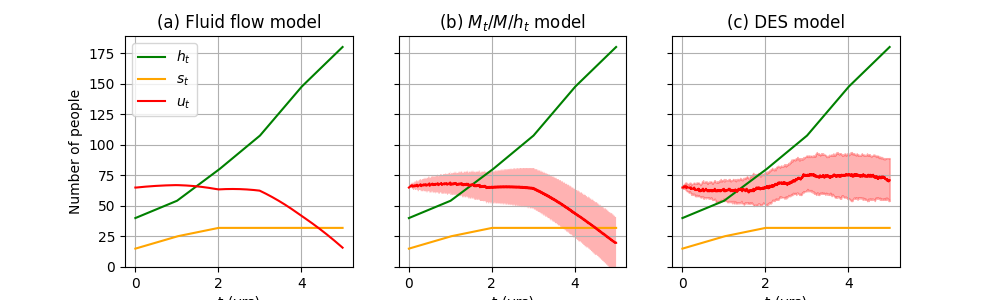
\includegraphics[scale=0.8]{u_t_example.png}
    \caption{Dynamics of $u_d$, $s^D_d$ and $h^D_d$. $n_0 = 12000$, $\mu_0 = 6.106 \times 10^{-4}$, Daily arrival rates $\lambda_d$ in each year: $10.0,11.9,13.1,13.1,11.8$.}
    \label{fig:ut-illustrative}
\end{figure}
%
Figure \ref{fig:ut-illustrative} shows an example of how one might come close to reaching zero unsheltered homelessness in five years.  The level of housing investment steadily increases over time.  There is some initial increase in shelter, though in general there is less investment in shelter over the long term than in housing.  The unsheltered population is stabilized and then eventually decreases approaching zero.  The arrival rates $\lambda_d$ are projected based on a current estimate of 10/day, along with the assumption that arrivals will increase in the coming years due to repercussions of COVID-19.  Eventually, prevention methods will take effect and the arrival rate will hopefully decline \citep{hometogether2022}. The daily service rate $\mu_0$ is equivalent to the mean of a triangular distribution with lower limit $0 \text{ weeks}$, upper limit $400 \text{ weeks}$ and mode $300 \text{ weeks}$.

In Section \ref{do} we will evaluate (\ref{u_t_discrete}) using annual housing and shelter capacity vectors $\boldsymbol{h} = \{h_t \hspace{0.1cm} \forall t \in 0,...,T\}$ and $\boldsymbol{s} = \{s_t \hspace{0.1cm} \forall t \in 0,...,T\}$ where $T$ is a time horizon in years. In this case we assume that any annual increase or decrease in capacity is spread evenly throughout the year, and (\ref{u_t_discrete}) becomes
%
\begin{align} \label{u_t_discrete_h_s_dependent}
u_d(\boldsymbol{h},\boldsymbol{s}) & = X_0 + \sum_{d'=1}^{d} \lambda_{d'} \delta t - \sum_{d'=1}^{d} \mu_0 h^D_{d'}(\boldsymbol{h}) \delta t - h^D_d(\boldsymbol{h}) - s^D_d(\boldsymbol{s}),
\end{align}
%
where 
%
\begin{align} \label{h_d}
h^D_d(\boldsymbol{h}) & = h_{\lfloor{\frac{d}{365}}\rfloor} + \frac{d-\lfloor\frac{d}{365}\rfloor}{365}(h_{\lceil{\frac{d}{365}}\rceil}-h_{\lfloor{\frac{d}{365}}\rfloor})
\end{align}
%
and
%
\begin{align} \label{s_d}
s^D_d(\boldsymbol{s}) & = s_{\lfloor{\frac{d}{365}}\rfloor} + \frac{d-\lfloor\frac{d}{365}\rfloor}{365}(s_{\lceil{\frac{d}{365}}\rceil}-s_{\lfloor{\frac{d}{365}}\rfloor}).
\end{align}
%
This fluid flow model has the advantage of being computationally cheap to run. It is also flexible to incorporate certain real-world system complexities. For example, we could model heterogeneous customer groups in different compartments with different servers, arrival rates and service rates. We could also incorporate re-entries to the system by applying an appropriate discount factor to the third term in Equation \ref{u_t_discrete_h_s_dependent}. 

\subsection{$M_t/M/h_t$ queueing model}
%
With an $M_t/M/h_t$ queueing model, where $h_t$ is the time-dependent number of housing servers, we are still modelling the system as illustrated in Figure \ref{fig:simple-q} but we no longer treat arrivals and departures as a fluid, but as individual people. We introduce stochasticity and would like to compute the probability distribution for the number of people housed, sheltered and unsheltered, throughout the time horizon. In doing so we allow a non-zero probability of their being $0$ people in the housing, thus relaxing the server-always-busy asumption we made with the fluid flow model.

Given the memoryless property of the exponential inter-arrival and service times in an $M_t/M/h_t$ queue, we can discretise time and treat this queue as a discrete-time Markov chain where the state space represents the number of people in the system and some large but finite $N$ is the largest possible state. With sufficiently small time intervals of length $\Delta t$, we can assume that within each interval the arrival rate is constant, the number of servers is constant and at most one state change can occur. Therefore, if we know the initial probabilities $p_n(t=0)$ of being in all states $n \in \{0,1,...,N\}$ then for all times $t \in \{0, \Delta t,...,T-\Delta t\}$, we can calculate the probabilities $p_n(t + \Delta t)$ as: 
% 
\begin{align*}
  p_n(t+\Delta t) = & \hspace{0.1cm} p_{n}(t)[1-\lambda(t)\Delta t-\mu_0 m_n(t) \Delta t] \\
                    & + p_{n+1}(t)[\mu_0 m_{n+1}(t) \Delta t] \\
                    & + p_{n-1}(t)[\lambda(t) \Delta t] \\
                    & + \hspace{0.1cm} o(\Delta t) \hspace{1cm} 1 \leq n \leq N-1
\end{align*}
% 
\begin{align*}
  p_0(t+\Delta t) = & \hspace{0.1cm} p_{0}(t)[1-\lambda(t)\Delta t] \\
                    & + p_{1}(t)[\mu_0 m_{1}(t) \Delta t] \\
                    & + \hspace{0.1cm} o(\Delta t)
\end{align*}
% 
\begin{align*}
  p_N(t+\Delta t) = & \hspace{0.1cm} p_{N}(t)[1-\mu_0 m_N(t) \Delta t] \\
                    & + p_{N-1}(t)[\lambda(t) \Delta t] \\
                    & + \hspace{0.1cm} o(\Delta t)
\end{align*}
% 
where $\lambda(t)$ is the arrival rate at time $t$, $\mu_0$ is the service rate of a single housing server and $m_n(t) = \min(n,h(t))$ is the number of busy housing servers when the system is in state $n$ at time $t$. The bias in the results introduced by using constant values in each time interval for $\lambda(t)$ and $h(t)$ vanishes as $\Delta t \to 0$. The probabilities $p_n(t)$ can then be analysed to estimate the expected number of people housed, sheltered and unsheltered, throughout the time horizon. For example, the expected number unsheltered at time $t$ is given by:

\begin{align} \label{u_t_mmt}
\mathbb{E}[u_t] & = \sum_{n=0}^{N} p_n(t) \max(0,n-h_t-s_t), 
\end{align}

where $s_t$ is the time-dependent number of shelters. This model is more computationally costly than the fluid flow model, but still cheap compared to a discrete-event simulation model. We have introduced stochasticity and allowed housing servers to be empty with some positive probability, but we are still limited in what real-world complexity we can model. Our choice of distribution for inter-arrival times and service times is also limited to the exponential distribution. 

\subsection{Discrete-event simulation model} \label{DES}
%
Discrete-event simulation (DES) is a form of stochastic simulation which models the evolution of a complex system according to a chronological event list which is updated throughout the simulation. DES is a powerful modeling tool given its ability to incorporate bespoke system complexities. It also naturally accomodates stochasticity by using a stream of $\text{Uniform}(\text{min} = 0, \text{max} = 1)$ pseudo-random numbers to drive the generation of random variates for model variables such as inter-arrival and service times. The drawback of DES is its computational cost which arises from the need to step through each event which occurs within the modelled system over the time horizon.

We have developed a DES model of our homelessness care system, which is a Python version of the DES model of \cite{singham2023discrete}, built in Simio. In this model, shelter acts as a server, giving rise to a tandem queueing system, as illustrated in Figure \ref{fig:des-q}. A proportion of those leaving housing re-enter the system, as illustrated, and the exponential and triangle distributions are used for inter-arrival and housing service times, respectively. 
%
\tikzstyle{server_s} = [rectangle, rounded corners, minimum width=0.5cm, minimum height=1cm,text centered, draw=black, fill=gray!30]
\tikzstyle{server_h} = [rectangle, rounded corners, minimum width=0.5cm, minimum height=1cm,text centered, draw=black, fill=teal!30]
\tikzstyle{arrow} = [thick,->,>=stealth]
%
\begin{figure}
  \begin{center}
    \begin{tikzpicture}
      \node (start) [empty, align=center] {};
      \node (shelter) [server_s, right of=start, xshift=3cm] {Shelter};
      \node (housing) [server_h, right of=shelter, xshift=3cm] {Housing};
      \node (end) [empty, right of=housing, xshift=1.4cm, align=center] {};
      \draw [arrow] (start) -- node [above] {Unsheltered} (shelter);
      \draw [arrow] (shelter) -- node [above] {Zero buffer}(housing);
      \draw [arrow] (housing) -- node [above] {}(end);
      \draw [arrow] (housing) to [out=210,in=330] node [below] {Partial re-entry}(shelter);
    \end{tikzpicture}
    \caption{Tandem queueing system with re-entries} \label{fig:des-q}
  \end{center}
\end{figure}

While this is still a relatively simple DES model, it provides the framework for us to add many more system complexities should we so desire. For example, we could model the non-zero time needed to occupy a house with a new resident following the departure of its previous resident. We could also model the process of conversion of shelter to housing, which is a strategy proposed by Alameda County to improve services in the long term. We thus treat our DES model as a high-fidelity model, capable of the highest level of modelling accuracy, in comparison to our low- and medium-fidelity models, albeit at a computational cost.

\newpage

\section{Deterministic optimisation with low-fidelity model} \label{do}
%
In this section, we will present an optimization formulation applied to our deterministic fluid flow model. This formulation will optimise the levels of housing and shelter to be built over time, and the objective function will attempt to minimise the unsheltered and sheltered population over the modelling horizon. Aside from the obvious need for cost constraints, we improve the real-world feasibility of our solutions by incorporating policy-based shape constraints on the housing and shelter capacities, which are a function of time. For example, though it would better from a queueing standpoint to spend all financial resources upfront, the reality is that investment from the taxpayer will likely ramp up over a period of years. Furthermore, though their is political appetite for the use of emergency shelter in the short term, this is not seen as a sustainable long-term solution, so we introduce a unimodal shape constraint on the shelter capacity function.
%
\subsection{Optimisation formulation} \label{opt}
%
First, we present the basic notation associated with the terms in our formulation. The associated numerical results will be presented in Section \ref{results}. We define the following terms:

\begin{itemize}
\item Let subscript $d$ denote time in days and subscript $t$ denote time in years.
\item Let $T_a$ be the horizon (in years) over which we model the dynamics of the system while altering housing and shelter capacities, where $T_a \in \mathbb{N}$. %\LRL{Could use $\mathbb{N}$ instead of $Z^+$.} \GB{Done}
\item Let $T_b$ be the additional horizon (in years) over which we continue to model the dynamics of the system without altering housing or shelter capacities, where $T_b \in \mathbb{N}$. We do this in order to allow increased housing capacity to have a meaningful effect on the system over a long period of time beyond a finite investment period. %\LRL{Should we have an explicit statement about why we continue to study the system on a time horizon beyond our decision making horizon? Otherwise it might seem like a slightly odd thing to do.} \GB{Done}
\item Let $D=(T_a+T_b)\times365$ be the total modeling horizon in days.
\item The vectors $\boldsymbol{h} = \{h_t \hspace{0.1cm} \forall t \in 0,...,T_a+T_b\}$ and $\boldsymbol{s} = \{s_t \hspace{0.1cm} \forall t \in 0,...,T_a+T_b\}$ are the model decision variables which contain continuous-valued annual housing and shelter capacities, respectively. The fluid flow model spreads annual changes in capacity equally over each day in the year, as detailed in equations (\ref{h_d}) and (\ref{s_d}).
\item $C$ is the total budget for building housing and shelter. \par
\item Let $c_h$ and $c_s$ be the costs of increasing $h_t$ and $s_t$, respectively, by 1, at any time.
\item Let $H_0$ and $S_0$ be the initial housing and shelter capacities, respectively.
\item Define $w \in (0,1)$ as a weight between two objective terms which ensures that a sheltered queue is not penalized more than an unsheltered queue of the same size.
\end{itemize}

Recall that $u_d$ and $s_d$ are the output of the fluid flow model reporting the unsheltered and sheltered populations each day, respectively.  Let $y(\boldsymbol{h},\boldsymbol{s})$ be a deterministic quadratic objective function, evaluated using the fluid flow model equations (\ref{u_t_discrete_h_s_dependent}), (\ref{h_d}) and (\ref{s_d}). We use a quadratic objective function to reflect the fact that neither the unsheltered nor the sheltered queue should become excessively long. Finding this balance involves a careful trade-off between building shelter (which quickly reduces the unsheltered queue) and building housing (which gives long term relief to the system, at the expense of initially large unsheltered queues). Furthermore, as seen in Alameda County, long waiting times can increase subsequent service times as people's situations may deteriorate. This further motivates the quadratic penalty on both parts of the queue.
%
\begin{align} \label{y}
  y(\boldsymbol{h},\boldsymbol{s}) = \frac{1}{D} \sum_{d=1}^{D} u_d(\boldsymbol{h},\boldsymbol{s})^2 + \frac{w}{D} \sum_{d=1}^{D} s^D_d(\boldsymbol{s})^2.  
\end{align}
%
We now introduce policy-based shape constraints. First, we ensure that the rate of housing capacity increase must stay the same or increase over $T_a$ to reflect the fact that budget available for housing capacity expansion may typically grow over time and not all be available immediately. This not only requires housing to increase over time, but the rate of change must increase as well, which amounts to an increasing derivative shape constraint.

We can also require shelter investment to follow a unimodal function, whereby it increases for a given time period, and then decreases.  This shape constraint has been suggested by Alameda County as a way of encouraging an initial ramp-up of shelter, but eventually excess shelter could be converted to housing to avoid permanent large shelters once the queue has been reduced.  To implement this unimodality constraint on $s_t$, we introduce a mode $T_c$ for the shelter capacity function over time, where $T_c \leq T_a$ and $T_c \in \mathbb{N}$. We ensure that the shelter capacity monotonically increases before $T_c$ and monotonically decreases subsequently. Decreases in the shelter capacity correspond to shelter being decomissioned - in this case the money saved may be spent on housing. The non-linear formulation including this unimodal shape constraint and rate of change constraint is:
%
\begin{eqnarray}
        \Phi = & \min_{\boldsymbol{h},\boldsymbol{s}} & y(\boldsymbol{h},\boldsymbol{s})\label{p2c0} \\
        \text{ s.t. } & \sum_{t=1}^{t'} c_{h}[h_{t}-h_{t-1}] + c_{s}[s_t-s_{t-1}] \leq C & \forall t' \in \{1, ..., T_a\}\,\quad \quad\label{p2c1}\\
        & h_0 = H_0 & \label{p2c2} \\
        & h_{t} \geq h_{t-1} & \forall t \in \{1,...,T_a\}\, \quad \quad\label{p2c3}\\   
        & h_t = h_{T_a} & \forall t \in \{T_a+1,...,T_a+T_b\}\, \quad \quad \label{p2c4} \\
        & h_{t+1} - h_{t} \geq h_{t} - h_{t-1} & \forall t \in \{1,...,T_a-1\}\, \quad \quad\label{p2c5} \\    
        & s_0 = S_0 & \label{p2c6} \\
        & s_{t} \geq s_{t-1} & \forall t \in \{1,...,T_c\}\, \quad \quad\label{p2c7} \\
        & s_{t} \leq s_{t-1} & \forall t \in \{T_c+1,...,T_a\}\, \quad \quad\label{p2c8} \\ 
        & s_t \geq s_0 & \forall t \in \{T_c+1, ..., T_a\}\, \quad \quad \label{p2c9} \\
        & s_t = s_{T_a} & \forall t \in \{T_a+1,...,T_a+T_b\}. \quad \quad \label{p2c10}
\end{eqnarray}
%
Constraints (\ref{p2c1}) ensure the total budget is never exceeded. A single budget constraint is not enough, since then the total budget could be exceeded in one year as long as a saving was subsequently made from decommissioning shelter. With this set of constraints we ensure that at no point can the total expenditure to that point exceed the total budget, so any savings from decommissioning shelter cannot be spent before they are made. Constraints (\ref{p2c2}) and (\ref{p2c6}) enforce the initial housing and shelter capacities. Constraints (\ref{p2c3}) ensure the housing capacity monotonically increases, while constraints (\ref{p2c5}) ensure the rate of change of housing capacity also monotonically increases from year to year. Constraints (\ref{p2c7}) ensure the shelter capacity monotonically increases up to the mode $T_c$ and constraints (\ref{p2c8}) ensure it subsequently decreases monotonically. Constraints (\ref{p2c9}) ensure the shelter capacity never drops below its initial capacity. Finally, constraints (\ref{p2c4}) and (\ref{p2c10}) fix $h_t$ and $s_t$ during the horizon $T_b$ after the building horizon has occurred.
%
\subsection{Numerical results} \label{results}

In Table \ref{tab:model_params} we list the model parameters we used when optimising formulations $\Phi$. These approximate values are taken from \cite{hometogether2022} and \cite{singham2023discrete}. We choose $w$ to be sufficiently high to give a meaningful penalty to shelter but without undermining its advantage over an unsheltered queue. Additionally, while we use a current estimate of the arrival rate of 10/day for the first $T_a$ years of the modeling horizon, we anticipate with major local prevention efforts \citep{RICActionPlan}, the arrival rate could potentially drop significantly to an estimate of 6/day.

\begin{table}
        \begin{center}
        \caption{Model parameters}
        \begin{tabular}{ |c|c| } 
         \hline
         \textbf{Parameter} & \textbf{Value ($\Phi$)}\\ 
         \hline
         $T_a$ & $5 \text{ years}$\\ 
         \hline
         $T_b$ & $5 \text{ years}$\\
         \hline
         $T_c$ & $3 \text{ years}$\\          
         \hline
         $\lambda_d$ & $\frac{10}{day} \hspace{0.1cm} \forall d \in \{1,...,T_a\times365\}$\\ 
          & $\frac{6}{day} \hspace{0.1cm} \forall d \in \{T_a\times365+1,...,D\}$\\          
         \hline           
         $X_0$ & 12,000 people\\         
         \hline
         $h_0$ & 4,000 units\\ 
         \hline
         $s_0$ & 1,500 units\\ 
         \hline      
         $c_h$ & 30,000 USD/unit\\ 
         \hline
         $c_s$ & 10,000 USD/unit\\ 
         \hline         
         $C$ & 200,000,000 USD\\ 
         \hline  
         $\mu_0$ & $6.106 \times 10^{-4}$/day \\ 
         \hline
         $w$ & $0.3$\\ 
         \hline
        \end{tabular}
        \label{tab:model_params}
        \end{center}
        \end{table}

In Figure \ref{fig:phi2opt} we illustrate the model dynamics for the optimal solution to $\Phi$, which involves the building of a mixture of extra housing and extra shelter. The quadratic penalty associated with a high unsheltered population encourages shelter which quickly reduces the size of the unsheltered queue. However, the quadratic penalty of having a large sheltered population encourages investment in housing. This housing investment in time also has a meaningful effect on reducing the unsheltered queue, since sufficient houses may be built to have a total service rate higher than the arrival rate, thus bringing stability to the system. 
%
\begin{figure}[h!]
    \centering
    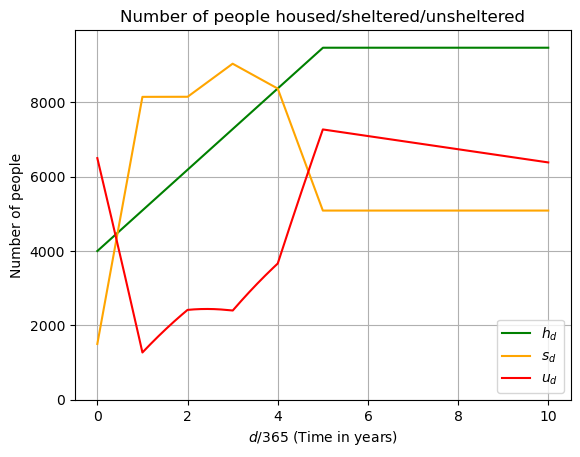
\includegraphics[scale=0.8]{phi2-opt.png}
    \caption{Optimal solution for $\Phi$.}
    \label{fig:phi2opt}
\end{figure}

We can see the effect of shape constraints. We note that the initial ramp up of shelter is able to bring the unsheltered queue down in the short term. The rate of increase in the housing capacity must not decrease over time so we see a more steady increase in housing compared to previous solutions. The total amount of housing we can build is affected by the fact that after the shelter mode at $t=3$ years, decommissioning shelter makes more budget available for housing. Thus we are able to achieve sufficient housing for a stable system in the long-term, while affording immediate relief to the system via shelter. We note that with this formulation, for every $3$ shelters decommissioned, $1$ house may be acquired, resulting in $2$ people immediately rejoining the unsheltered part of the queue. Although this enables the housing capacity to increase which is good for long-term relief to the system, the immediate effect is undesirable in practice and we see that after $5$ years the unsheltered queue is again very large. An alternative formulation may enforce a more controlled decommissioning process by, for example, including a shape constraint on the total number of housing and shelter units.      
\begin{figure}[h!]
    \centering
    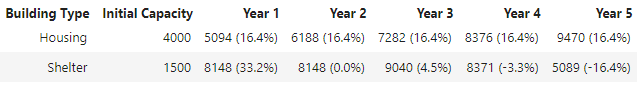
\includegraphics[scale=0.8]{results_comparison.png}
    \caption{Optimal capacity per year (Proportion of total budget spent per year)}
    \label{tab:phi1phi2results}
\end{figure}

In Figure \ref{tab:phi1phi2results} we detail the optimal solution to $\Phi$ in terms of the capacity at the end of each year and the proportion of the total budget spent on building in that year. Negative budget spent corresponds to a saving made by decommissioning shelter. The optimal solution spends the maximum possible budget of 200,000,000 USD. The solution sees a large early ramp up of shelter and a steady investment in housing over time. In years $4$ and $5$ we see decommissioning of shelter to enable the continued investment in housing. 

We solved this problem in $0.759$ seconds using the IPOPT solver in Pyomo. All code used for this analysis is publicly available \href{https://github.com/grahamburgess3/psor-paper-housing}{on GitHub}.

\subsection{Determinsitic optimisation: discussion} \label{do-discuss}

Most capacity planning formulations we have reviewed in the literature consider capacity expansion from a single-stage perspective, in that the decision-maker has one shot to choose and optimize a fixed capacity to accommodate the queueing system.   In reality, most public sector services do not have the resources to instantaneously ramp up to the ideal capacity, as there may be budgetary or time constraints that control this rate.  A model that accounts for these limits in capacity expansion over time will provide a more realistic and executable plan, hence we attempt to provide a method for determining how to allocate resources over time.

While housing is the primary resource and is modeled as the main server system, we also model investment into shelter, which supports some of the people in the queue, while not modeled as a server. Our quadratic objective function is able to balance the desire for high levels of housing at high cost against cheaper shelter options. In addition to budgetary constraints, we employ shape constraints as a means of ensuring our investment function output is feasible from a policy-making and implementation standpoint.  The idea of a unimodal function for shelter investment has been suggested by Alameda County, and such shape constraints can easily be implemented in our framework.

There are many opportunities for alternative formulations.  Smoothness constraints on the unimodal shelter capacity function may give more practical solutions that appear reasonable to constituents. Further constraints to control the decommissioning of shelter may also be appropriate. A bi-objective formulation would likely give further insight into the trade-off between short-term relief to the system via shelter and long-term relief via housing. Alternatively, a goal programming formulation which penalised deviations from a time-dependent goal on the unsheltered population would be interesting to explore.

We have here performed deterministic optimisation using a low-fidelity fluid flow model. This has enabled us to develop and explore an optimisation formulation which captures the key objectives, trade offs and constraints. It has also enabled us to quickly get a feel for the nature of good solutions to the time-dependent capacity planning problem using a simple model. The natural next step is to develop a stochastic optimization model to account for parameter uncertainty.

\newpage

\section{Discussion of uncertainty} \label{uncert}

Our optimisation in Section \ref{do} assumes that we know the future arrival rates of homeless people into the homeless care system, and that we know their service times in housing. The fluid flow model projects forward the resulting unsheltered queue based on these exact quantities. In reality, actual inter-arrival times (or service times) are realisations of some unknown true distribution which we can only estimate using information available to us. Even if we knew the true distributions, we would not know what the next inter-arrival time (or service time) would be, due to the random nature of these processes. It is important that we consider these aspects of uncertainty as we move forward to consider simulation optimisation.

As discussed in Section \ref{models}, a stochastic simulation model offers a high-fidelity model of the homeless care system. It incorporates the stochasticity in inter-arrival and service times, and it allows us to capture certain important real-world complexities, such as the conversion of shelter to housing. There are two types of uncertainty in stochastic simulation: input uncertainty and stochastic uncertainty. Input uncertainty arises from not knowing the true input models for, say, inter-arrival and service times. Stochastic uncertainty arises from only ever simulating a finite amount of random variates from the input models used. The latter can be mitigated by performing many simulation replications. The former is typically mitigated by bootstrapping from the data used to fit the input models, to fit new input models which can be used to generate new random variates in new simulation replications.

Simulation optimisation suffers from both input uncertainty and stochastic uncertainty as a direct result of using stochastic simulation to model the performance of a solution. The main focus of this PhD research, at least initially, will be multi-fidelity simulation optimisation where we do not consider the effects of input uncertainty. I.e. we assume that we know the true distributions for inter-arrival times and service times. We do, of course, consider stochastic uncertainty: i.e. given known input models, with a finite comptuational budget we can only estimate the performance of a solution. We will endeavour to use multi-fidelity models alongside stochastic simulation so as to identify optimal or close to optimal solutions in a computationally efficient way, given the inherent stochastic uncertainty.

We do here acknowledge that for the homeless care system, there are extremely high levels of input uncertainty. Even if we fitted an input model for inter-arrival times using an extensive dataset of inter-arrival times of homeless people in recent years, we would still be highly uncertain of whether this model would accurately predict future inter-arrival times because the future is full of unknowns. It is simply impossible to predict future inter-arrival times because they are connected with many other events which are highly unpredictable, such as house prices, political decisions and global health and climate emergencies. Our decision to not consider input uncertainty is therefore not without due consideration. We anticipate that incorporating multi-fidelity models into simulation optimisation is challenging enough without input uncertainty. Once we have made progress with this, we will consider how our methodology could be adapted to consider input uncertainty. To this end, we may first consider simulation optimisation with high input uncertainty, without incorporating multi-fidelity models. This in itself is an active area of research.

\newpage

\section{Potential contributions at intersection of integer-ordered and multi fidelity SO} \label{mfso}

\begin{itemize}[noitemsep]
\item Using low-fidelity models to quickly compute gradients in RSPLINE/DSA.
\item Adding prior information to GMRF using low-fidelity model.
\item Modelling errors of low fidelity models using GMRF.
\end{itemize}

\newpage

\section{Conclusion}\label{conc}

\newpage

\bibliographystyle{apalike}
\bibliography{bibliography.bib}

\end{document}